\begin{name}
	{\tenchude}
	{\tendethi}
	{Sở Hải Phòng}
	{\thoigian}
\end{name}
\Opensolutionfile{ans}[ans/2-TT-SoHaiPhong-L1-NH21-22]


\begin{ex}%[Dự án 016-2-TT-SoHaiPhong-L1-NH21-22-Manda La]%[2H2Y1-1]
Thể tích $V$ của khối trụ có bán kính $r$ và chiều cao $h$ được tính theo công thức nào dưới đây?
\choice
{\True $V=\pi r^2h$}
{ $V=\dfrac{1}{3}\pi r^2h$}
{ $V=\pi rh^2$}
{ $V=r^2h$}
\loigiai{
Theo công thức tính thể tích khối trụ ta có $V=\pi r^2h$.}
\end{ex}

\begin{ex}%[Dự án 016-2-TT-SoHaiPhong-L1-NH21-22-Manda La]%[2D3K2-4]
Cho hàm số $y=f( x )$ có đạo hàm liên tục trên $\mathbb{R}$, đồ thị của $y=f( x )$ đi qua điểm $A( 1;0 )$ và $f( 4-x )+f( x )=4,\forall x\in \mathbb{R}$. Tích phân $\displaystyle\int\limits_1^3 x( x-2 )\left[ f( x )+f'( x ) \right]\mathrm{~d}x $ bằng
\choice
{ $-\dfrac{16}{3}$}
{ $\dfrac{8}{3}$}
{\True $\dfrac{16}{3}$}
{ $\dfrac{-8}{3}$}
\loigiai{
Ta chọn hàm số $y=ax+b$.\\
Đồ thị của $y=f( x )$ đi qua điểm $A( 1;0 )$ nên $a+b=0.\quad ( 1 )$\\
Từ $f( 4-x )+f( x )=4,\forall x\in \mathbb{R}$, thay $x=1$ vào ta có $f( 3 )+f( 1 )=4\Leftrightarrow f( 3 )=4$.\\
Suy ra đồ thị của $y=f( x )$ đi qua điểm $B( 3;4 )$ nên $3a+b=4.\quad ( 2 )$\\
Từ $( 1 )\And ( 2 )$ ta có hệ phương trình $\left\{ \begin{aligned}
& a+b=0 \\
& 3a+b=4 \\
\end{aligned} \right.\Leftrightarrow \left\{ \begin{aligned}
& a=2 \\
& b=-2 \\
\end{aligned} \right.\Rightarrow f( x )=2x-2;f'( x )=2$.\\
Vậy tích phân $\displaystyle\int\limits_1^3 x( x-2 )\left[ f( x )+f'( x ) \right]\mathrm{~d}x =\displaystyle\int\limits_1^3 x( x-2 )2x\mathrm{~d}x =\displaystyle\int\limits_1^3 ( 2x^3-4x^2 )\mathrm{~d}x =\dfrac{16}{3}$.}
\end{ex}

\begin{ex}%[Dự án 016-2-TT-SoHaiPhong-L1-NH21-22-Manda La]%[2H2Y2-1]
Cho hình cầu có bán kính bằng $r$. Diện tích $S$ của hình cầu đã cho được tính theo công thức nào dưới đây?
\choice
{\True $S=4\pi r^2$}
{ $S=4r^2$}
{ $S=2\pi r^2$}
{ $S=\dfrac{4}{3}\pi r^2$}
\loigiai{
Công thức tính diện tích $S$ của hình cầu là $S=4\pi r^2$.
}
\end{ex}

\begin{ex}%[Dự án 016-2-TT-SoHaiPhong-L1-NH21-22-Manda La]%[2H1Y3-2]
Cho khối hộp chữ nhật có chiều dài, chiều rộng, chiều cao lần lượt bằng $a,b,c$. Thể tích $V$ của khối hộp chữ nhật đã cho được tính theo công thức nào dưới đây?
\choice
{ $V=\dfrac{1}{3}abc$}
{ $V=\dfrac{1}{6}abc$}
{\True $V=abc$}
{ $V=2abc$}
\loigiai{
Ta có $V=B\cdot h=( ab )\cdot c=abc$.
}
\end{ex}

\begin{ex}%[Dự án 016-2-TT-SoHaiPhong-L1-NH21-22-Manda La]%[2D1B5-1]
\immini{
Cho đồ thị hàm số $y=ax^3+bx^2+cx+d$ có đồ thị như hình vẽ.\\
%	\centerline{\includegraphics{hinh/THVBA29052241157THVBAimage3EX}}\\
Xác định dấu của các hệ số $a,b,c$.
\choice
{ $\left\{ \begin{aligned}
& a<0 \\
& b<0 \\
& c<0 \\
\end{aligned} \right.$}
{ $\left\{ \begin{aligned}
& a<0 \\
& b>0 \\
& c=0 \\
\end{aligned} \right.$}
{ $\left\{ \begin{aligned}
& a<0 \\
& b>0 \\
& c>0 \\
\end{aligned} \right.$}
{\True $\left\{ \begin{aligned}
& a<0 \\
& b>0 \\
& c<0 \\
\end{aligned} \right.$}
}{
\begin{tikzpicture}[scale=0.8,>=stealth, font=\footnotesize, line join=round, line cap=round]
\def\a{-1} \def\b{3.55} \def\c{-3} \def\d{-0.3} % Hệ số
\def\xmin{-1.5} \def\xmax{4}
\def\ymin{-1.6} \def\ymax{4}
%	\draw[color=gray!50,dashed] (\xmin,\ymin) grid (\xmax,\ymax);
\draw[->] (\xmin,0)--(\xmax,0) node [below]{$x$};
\draw[->] (0,\ymin)--(0,\ymax) node [right]{$y$};
\node at (0,0) [below left]{$O$};
\clip (\xmin+0.1,\ymin+0.1) rectangle (\xmax-0.5,\ymax-0.1);
\draw[smooth,samples=300] plot(\x,{\a*(\x-0.27)^3+\b*(\x-0.2)^2+\c*(\x-0.6)+\d});
\end{tikzpicture}
}
\loigiai{
Nhìn đồ thị ta thấy với $x=0\Rightarrow y=d>0$.\\
Hai điểm cực trị có hoành độ dương nên $\left\{ \begin{aligned}
& x_1+x_2=-\dfrac{2b}{3a}>0 \\
& x_1\cdot x_2=\dfrac{c}{3a}>0. \\
\end{aligned} \right.$\\
Vì$\lim\limits_{x\to +\infty } y=-\infty $ nên $a<0\Rightarrow b>0,c<0$.
}
\end{ex}

\begin{ex}%[Dự án 016-2-TT-SoHaiPhong-L1-NH21-22-Manda La]%[2H3Y3-1]
Trong không gian với hệ trục tọa độ $Oxyz$, đường thẳng $d\colon\left\{ \begin{aligned}
& x=1-t \\
& y=2+2t \\
& z=3-t \\
\end{aligned} \right.$ có một véc-tơ chỉ phương là
\choice
{ $\overrightarrow {u}_3=( 1;-2;-1 )$}
{\True $\overrightarrow {u}_2=( 1;-2;1 )$}
{ $\overrightarrow {u}_1=( 1;2;1 )$}
{ $\overrightarrow {u}_4=( 1;2;3 )$}
\loigiai{
Đường thẳng $d\colon\left\{ \begin{aligned}
& x=1-t \\
& y=2+2t \\
& z=3-t \\
\end{aligned} \right.$ có một vectơ chỉ phương là $\overrightarrow{u}=( 1;-2;1 )$.
}
\end{ex}

\begin{ex}%[Dự án 016-2-TT-SoHaiPhong-L1-NH21-22-Manda La]%[2D1Y4-1]
Đồ thị hàm số $y=\dfrac{3x+2}{x-2}$ có bao nhiêu đường tiệm cận?
\choice
{ $0$}
{ $3$}
{\True $2$}
{ $1$}
\loigiai{
Tập xác định $\mathscr{D}=\mathbb{R}\setminus \left\{ 2 \right\}$.\\
Ta có $\lim\limits_{x\to \pm \infty } \dfrac{3x+2}{x-2}=3\Rightarrow $ Đồ thị hàm số có đường tiệm cận ngang $y=3$.\\
Ta cũng có $\lim\limits_{x\to 2^{+}} \dfrac{3x+2}{x-2}=+\infty \Rightarrow $ Đồ thị hàm số có đường tiệm cận đứng $x=2$.\\
Vậy đồ thị hàm số có $2$ đường tiệm cận.
}
\end{ex}
\begin{ex}%[Dự án 016-2-TT-SoHaiPhong-L1-NH21-22-Manda La]%[1D2B5-2]
Trong một hộp có $5$ viên bi màu đỏ, $4$ viên bi màu vàng và $3$ viên bi màu trắng (các viên bi cùng màu là phân biệt). Rút ngẫu nhiên ra $3$ viên bi, xác suất để $3$ viên bi rút ra có đủ $3$ màu bằng
\choice
{ $\dfrac{1}{22}$}
{ $\dfrac{3}{55}$}
{ $\dfrac{3}{22}$}
{\True $\dfrac{3}{11}$}
\loigiai{
Không gian mẫu $n( \Omega )=\mathrm{C}_{12}^3$.\\
Gọi biến cố $A\colon$ \lq\lq $3$ viên bi rút ra có đủ $3$ màu\rq\rq.\\
Số cách chọn $3$ viên bi có đủ $3$ màu là $\mathrm {C}_5^1\cdot\mathrm {C}_4^1\cdot\mathrm {C}_3^1=60$ cách.\\
Suy ra $ n( A )=60 $.\\
Vậy  Xác suất để $3 $ viên bi rút ra có đủ $3$ màu là $\mathrm{P}( A )=\dfrac{n( \Omega )}{n( A )}=\dfrac{3}{11}\cdot$}
\end{ex}

\begin{ex}%[Dự án 016-2-TT-SoHaiPhong-L1-NH21-22-Manda La]%[2H3Y1-2]
Trong không gian với hệ trục tọa độ $Oxyz$, cho hai véc-tơ $\overrightarrow{u}=( 1;3;-2 )$ và $\overrightarrow{v}=( 0;1;2 )$. Khi đó $\overrightarrow{u}\cdot\overrightarrow{v}$ bằng
\choice
{ $0$}
{\True $-1$}
{ $1$}
{ $-2$}
\loigiai{
Tích vô hướng $\overrightarrow{u}\cdot\overrightarrow{v}=1\cdot0+3\cdot1+( -2 )\cdot2=-1$.
}
\end{ex}

\begin{ex}%[Dự án 016-2-TT-SoHaiPhong-L1-NH21-22-Manda La]%[2D1B3-1]
Giá trị lớn nhất của hàm số $y=4x-x^2,x\in [ 0\,;4 ]$ bằng
\choice
{\True $4$}
{ $2$}
{ $8$}
{ $0$}
\loigiai{
Ta có $y'=4-2x\,;\,y'=0\Leftrightarrow 4-2x=0\Leftrightarrow x=2$.\\
Tính các giá trị ta được $y( 0 )=0$;	$y( 4 )=0$ và	$y( 2 )=4$.\\
Vậy $ \max\limits_{x\in \left[ 0;4 \right]} y=4$.
}
\end{ex}

\begin{ex}%[Dự án 016-2-TT-SoHaiPhong-L1-NH21-22-Manda La]%[2D1B2-3]
Tìm bộ $3$ số $( a;b;c )$ để đồ thị hàm số $y=ax^4+bx^2+c$ có $A( 0;-3 )$ là điểm cực đại và $B( -1;-5 )$ là một điểm cực tiểu.
\choice
{ $( 2;4;-3 )$}
{ $( -3;-1;-5 )$}
{ $( -2;4;-3 )$}
{\True $( 2;-4;-3 )$}
\loigiai{
Ta có $y=f( x )=ax^4+bx^2+c\Rightarrow {y}'=f'( x )=4ax^3+2bx$.\\
Với $A( 0;-3 )$ là điểm cực đại và $B( -1;-5 )$ là một điểm cực tiểu ta có
\[\left\{ \begin{aligned}
& f( 0 )=-3 \\
& f( -1 )=-5 \\
& f'( -1 )=0 \\
\end{aligned} \right.\Leftrightarrow \left\{ \begin{aligned}
& a\cdot 0^4+b\cdot 0^2+c=-3 \\
& a( -1 )^4+b( -1 )^2+c=-5 \\
& 4a( -1 )^3+2b( -1 )=0 \\
\end{aligned} \right.\Leftrightarrow \left\{ \begin{aligned}
& a=2 \\
& b=-4 \\
& c=-3. \\
\end{aligned} \right.\]
Vậy bộ $3$ số $( a;b;c )$ là $( 2;-4;-3 )$.
}
\end{ex}

\begin{ex}%[Dự án 016-2-TT-SoHaiPhong-L1-NH21-22-Manda La]%[2H3Y1-3]
Trong không gian với hệ trục $Oxyz$, mặt cầu $( S )\colon ( x-a )^2+( y-b )^2+( z-c )^2=R^2$ có toạ độ tâm là
\choice
{\True $( a;b;c )$}
{ $\left( \dfrac{a}{2};\dfrac{b}{2};\dfrac{c}{2} \right)$}
{ $( -a;-b;-c )$}
{ $( 2a;2b;-2c )$}
\loigiai{
Mặt cầu $( S )\colon ( x-a )^2+( y-b )^2+( z-c )^2=R^2$ có toạ độ tâm là $( a;b;c )$.
}
\end{ex}

\begin{ex}%[Dự án 016-2-TT-SoHaiPhong-L1-NH21-22-Manda La]%[1H3B5-3]
Cho hình hộp chữ nhật $ABCD.{A}'{B}'{C}'{D}'$ có $AB=a,\,AD=2a,A{A}'=2a$. Khoảng cách từ điểm $A$ đến mặt phẳng $( {A}'BD )$ bằng
\choice
{ $\dfrac{a\sqrt{3}}{2}$}
{ $a$}
{\True $\dfrac{a\sqrt{6}}{3}$}
{ $\dfrac{a\sqrt{2}}{2}$}
\loigiai{
%\centerline{\includegraphics{hinh/THVBA29052241157THVBAimage2EX}}
\immini{
Trong $( ABCD )$, kẻ $AK\perp BD$.\\
Trong $( AO{A}' )$, kẻ $AH\perp {A}'K$.\\
Ta có $\left\{ \begin{aligned}
& AH\perp {A}'K \\
& AH\perp BD\, (\text{Vì}\, BD\perp ( {A}'AC ) ) \\
\end{aligned} \right.\Rightarrow AH\perp ( {A}'BD )$.
$$\left.\begin{aligned}[t]
\dfrac{1}{AH^2}=&\dfrac{1}{AK^2}+\dfrac{1}{A{{A}'}^2}\\
=&\dfrac{1}{A{{A}'}^2}+\dfrac{1}{AB^2}+\dfrac{1}{AD^2}\\
=&\dfrac{1}{a^2}+\dfrac{1}{( 2a )^2}+\dfrac{1}{( 2a )^2}\cdot
\end{aligned} \right.$$
Suy ra $ AH=\dfrac{a\sqrt{6}}{3}\cdot$
}{
\begin{tikzpicture}[scale=0.9,>=stealth, font=\footnotesize, line join=round, line cap=round]
\def\a{4.5}
\coordinate (D)at(0,0);
\coordinate (C)at (\a-0.2,0);
\coordinate(A)at (0.4*\a,0.4*\a);
\coordinate (B) at ($(A)+(C)-(D)$);
\coordinate (D') at ($(D)+(0,\a)$);
\coordinate (B') at ($(B)+(0,\a)$);
\coordinate (C') at ($(C)+(0,\a)$);
\coordinate (A') at ($(A)+(0,\a)$);
\draw ($(B)!0.38!(D)$) coordinate (K) ;
\draw ($(K)!0.38!(A')$) coordinate (H) ;
\draw  (D)--(C)--(B)--(B')--(A')--(D')--(C')--(B') (D)--(D') (C)--(C'); \draw[dashed](A)--(D)--(B)--(A)--(A')--(K)--(A)--(H) (D)--(A')--(B);
\foreach \d/\g in {A/160, B/20, C/-40, D'/170, C'/-40, B'/60, A'/100, D/-120, K/-45, H/10}
\path[draw=black,fill=black] (\d) circle(1pt) + (\g:9pt) node {$\d$};
\end{tikzpicture}}
}
\end{ex}

\begin{ex}%[Dự án 016-2-TT-SoHaiPhong-L1-NH21-22-Manda La]%[2D3B3-1]
Cho hàm số $y=f( x )$ liên tục trên $[ -5;5 ]$ và có đồ thị như hình vẽ
\begin{center}
\begin{tikzpicture}[scale=0.8,>=stealth, font=\footnotesize, line join=round, line cap=round]
\def\xmin{-5.5} \def\xmax{5.5}
\def\ymin{-2.5} \def\ymax{4.5}
\draw[->] (\xmin,0)--(\xmax,0) node [below]{$x$};
\draw[->] (0,\ymin)--(0,\ymax) node [left]{$y$};
\node at (0,0) [below right]{$O$};
\draw[line width=0.8] (-5,0)--(-2,-2)--(3,3)--(4,3)--(5,0);
\draw[dotted] (-5,0)node[below left]{$-5$} (-2,0)node[below left]{$-2$}--(-2,-2)--(0,-2)node[above left]{$-2$} (3,0)node[below left]{$3$}--(3,3)--(0,3)node[above left]{$3$} (4,3)--(4,0)node[below left]{$4$} (5,0)node[below left]{$5$};
\fill[black] (-5,0) circle (1pt) (-2,0) circle (1pt) (-2,-2) circle (1pt) (0,-2) circle (1pt)(0,0) circle (1pt)(3,0) circle (1pt)(3,3) circle (1pt)(0,3) circle (1pt)(4,3) circle (1pt)(4,0) circle (1pt)(5,0) circle (1pt);
\end{tikzpicture}
\end{center}
Tích phân $\displaystyle\int\limits_{-5}^{5} f( x )\mathrm{~d}x $ bằng
\choice
{ $8$}
{\True $4$}
{ $14$}
{ $19$}
\loigiai{
Ta có $\displaystyle\int\limits_{-5}^{5} f( x )\mathrm{~d}x =\displaystyle\int\limits_{-5}^{0} f( x )\mathrm{~d}x +\displaystyle\int\limits_{0}^{5} f( x )\mathrm{~d}x =-S_1+S_2$.\\
Với $S_1=\dfrac{1}{2}\cdot 2\cdot 5=5$ (một phần hai đường cao nhân cạnh đáy).\\
$S_2=\dfrac{( 1+5 )\cdot 3}{2}=9$ ( với $S_2$ là diện tích hình thang).\\
Vậy $\displaystyle\int\limits_{-5}^{5} f( x )\mathrm{~d}x =-S_1+S_2=-5+9=4.$
}
\end{ex}

\begin{ex}%[Dự án 016-2-TT-SoHaiPhong-L1-NH21-22-Manda La]%[2D4Y3-1]
Nghịch đảo của số phức $1+i$ là số phức
\choice
{ $-1+i$}
{ $1-i$}
{ $\dfrac{1}{2}+\dfrac{1}{2}i$}
{\True $\dfrac{1}{2}-\dfrac{1}{2}i$}
\loigiai{
Nghịch đảo của số phức $1+i$ là số phức  $\dfrac{1}{1+i}=\dfrac{1-i}{( 1+i )( 1-i )}=\dfrac{1-i}{2}=\dfrac{1}{2}-\dfrac{1}{2}i$.
}
\end{ex}

\begin{ex}%[Dự án 016-2-TT-SoHaiPhong-L1-NH21-22-Manda La]%[2D3Y1-1]
Họ nguyên hàm của hàm số $f( x )=a^x$ $( 1\ne a>0 )$ là
\choice
{ $\dfrac{a^x}{\log a}+C$}
{\True $\dfrac{a^x}{\ln a}+C$}
{ $\dfrac{a^{x+1}}{x+1}+C$}
{ $a^x\cdot \ln a+C$}
\loigiai{
Ta có $\displaystyle\int a^x\mathrm{~d}x= \dfrac{a^x}{\ln a}+C$.
}
\end{ex}

%câu 17
\begin{ex}%[DuAn16-SoHaiPhong-NguyenTruongVinh]%[2D3B2-1]
	Nếu $\displaystyle\int\limits_0^1{f( x )\textrm{ d}x}=a$ và $\displaystyle\int\limits_1^2{f( x )\textrm{ d}x}=b$ thì $\displaystyle\int\limits_0^2{f( x )\textrm{ d}x}$ bằng 
	\choice
	{$\dfrac{a+b}{2}$}
	{$b-a$ }
	{\True $a+b$}
	{$a-b$}
	\loigiai{
		Ta có $\displaystyle\int\limits_0^2{f( x )\textrm{ d}x}=\displaystyle\int\limits_0^1{f( x )\textrm{ d}x}+\displaystyle\int\limits_1^2{f( x )\textrm{ d}x}=a+b$.}
\end{ex}
%câu 18
\begin{ex}%[DuAn16-SoHaiPhong-NguyenTruongVinh]%[2D4B1-1]
	Có bao nhiêu số phức thỏa mãn $\left\{ \begin{aligned}
	& \left| z+\overline{z}-2 \right|+\left| z+\overline{z}-2i \right|=4 \\ 
	& \left| z-1 \right|=1 \\ 
	\end{aligned} \right. $ ?
	\choice
	{$4$}
	{$2$}
	{\True$3$}
	{$1$}
	\loigiai{
		Giả sử $z=a+bi\,;\,( a,\,b\in \mathbb{R} )$.\\
		Ta có $\left| z-1 \right|=1\Leftrightarrow \left| a+bi-1 \right|=1\Leftrightarrow {{( a-1 )}^2}+b^2=1$. (*)\\
		Ta có $\left| z+\overline{z}-2 \right|+\left| z+\overline{z}-2i \right|=4\\
		\Leftrightarrow \left| a+bi+a-bi-2 \right|+\left| a+bi+a-bi-2i \right|=4$\\
		$\Leftrightarrow \left| a-1 \right|+\left| a-i \right|=2\Leftrightarrow \left| a-1 \right|+\sqrt{a^2+1}=2\Leftrightarrow \sqrt{a^2+1}=2-\left| a-1 \right|$. (1)\\
		Trường hợp 1: $a\ge 1$. \\
		Phương trình (1) $\Leftrightarrow \sqrt{a^2+1}=3-a\Leftrightarrow \heva{
			& a\le 3 \\ 
			& a^2+1=9-6a+a^2 } \Leftrightarrow a=\dfrac{4}{3}\,\,(\text{thỏa mãn})$.\\
		Thay $a=\dfrac{4}{3}$ vào (*) có $b^2=\dfrac{8}{9}\Rightarrow \hoac{
			& b=\dfrac{2\sqrt{2}}{3} \\ 
			& b=-\dfrac{2\sqrt{2}}{3} }\Rightarrow \hoac{
			& z=\dfrac{4}{3}+\dfrac{2\sqrt{2}}{3}i \\ 
			& z=\dfrac{4}{3}-\dfrac{2\sqrt{2}}{3}i} $.\\
		Trường hợp 2: $a<1$. \\
		Phương trình (1) $\Leftrightarrow \sqrt{a^2+1}=a+1\Leftrightarrow \heva{
			& a\ge -1 \\ 
			& a^2+1=a^2+2a+1} 
		\Leftrightarrow a=0\,\,(\text{thỏa mãn})$.\\
		Thay $a=0$ vào (*) có $b=0$.
	}
\end{ex}
%câu 19
\begin{ex}%[DuAn16-SoHaiPhong-NguyenTruongVinh]%[2D4Y1-1]
	Cho số phức $z=a+bi\,;\,( a,\,b\in \mathbb{R} )$, khi đó mô-đun của số phức $z$ bằng
	\choice
	{$\sqrt{a^2-b^2}$ }
	{\True $\sqrt{a^2+b^2}$}
	{$\sqrt{a+b}$}
	{$\left| a+b \right|$}
	\loigiai{
		Ta có $z=a+bi\Rightarrow \left| z \right|\,=\sqrt{a^2+b^2}$.}
\end{ex}
%câu 20
\begin{ex}%[DuAn16-SoHaiPhong-NguyenTruongVinh]%[2D4Y1-1]
	Số phức liên hợp của số phức $z=2-3i$ là
	\choice
	{$-2-3i$}
	{\True $2+3i$}
	{$3+2i$}
	{$3-2i$}
	\loigiai{
		Số phức liên hợp của $z=2-3i\,$ là $\overline{z}=2+3i$.
	}
\end{ex}
%câu 21
\begin{ex}%[DuAn16-SoHaiPhong-NguyenTruongVinh]%[1D3Y4-1]
	Cho cấp số nhân $( u_n )$ với $u_1=1$ và công bội $q=2$. Tổng của $5$ số hạng đầu của cấp số nhân đã cho bằng 
	\choice
	{$32$ }
	{\True $31$}
	{$63$}
	{$64$}
	\loigiai{
		Ta có $\mathrm{S}_5=\dfrac{u_1( q^5-1 )}{q-1}=\dfrac{2^5-1}{2-1}=31$.}
\end{ex}
%câu 22
\begin{ex}%[DuAn16-SoHaiPhong-NguyenTruongVinh]%[2D3B2-1]
	Cho $F( x )$ là một nguyên hàm của hàm số $f( x )$. Biết rằng $F( 0 )=1$ và $\displaystyle\int\limits_0^1{f( x )} \text{\, d}x=2$, khi đó $F( 1 )$ bằng 
	\choice
	{$-1$}
	{$2$}
	{\True $3$}
	{$1$}
	\loigiai{
		Ta có $\displaystyle\int\limits_0^1{f( x )}\text{\,d}x=2\Leftrightarrow F( 1 )-F( 0 )=2\Leftrightarrow F( 1 )=2+1=3$.}
\end{ex}
%câu 23
\begin{ex}%[DuAn16-SoHaiPhong-NguyenTruongVinh]%[1D2Y2-1]
	Với $n$ là số nguyên dương, $k$ là số tự nhiên $( k\le n )$, công thức nào dưới đây \textbf{đúng}?
	\choice
	{$\mathrm{C}_n^k=k!( n-k )!$ }
	{$\mathrm{C}_n^k=\dfrac{n!}{( n-k )!}$}
	{\True $\mathrm{C}_n^k=\dfrac{n!}{k!( n-k )!}$ }
	{$\mathrm{C}_n^k=\dfrac{n!}{k!}$}
	\loigiai{
		Ta có $\mathrm{C}_n^k=\dfrac{n!}{k!( n-k )!}$.}
\end{ex}
%câu 24
\begin{ex}%[DuAn16-SoHaiPhong-NguyenTruongVinh]%[2H3Y2-2]
	Trong không gian với hệ tọa độ $Oxyz$, cho ba điểm $A( 2;0;0 )$, $B( 0;3;0 )$ và $C( 0;0;1 )$. Véc-tơ nào dưới đây là véc-tơ pháp tuyến của mặt phẳng $( ABC )$?
	\choice
	{$\overrightarrow{n_2}=( 2;3;1 )$}
	{$\overrightarrow{n_4}=( \dfrac{1}{3};\dfrac{1}{2};1 )$}
	{$\overrightarrow{n_3}=( 3;1;6 )$}
	{\True $\overrightarrow{n_1}=( 3;2;6 )$}
	\loigiai{
		Mặt phẳng $( ABC )$ có phương trình là $\dfrac{x}{2}+\dfrac{y}{3}+\dfrac{z}{1}=1\Leftrightarrow 3x+2y+6z-6=0$.\\
		Vậy mặt phẳng $( ABC )$ có một véc-tơ pháp tuyến là $\overrightarrow{n_1}=( 3;2;6 ).$}
\end{ex}
%câu 25
\begin{ex}%[DuAn16-SoHaiPhong-NguyenTruongVinh]%[2D2Y3-2] 
	Với hai số thực dương bất kì $a,b$. Mệnh đề nào dưới đây là đúng?
	\choice
	{$\ln ( ab )=\ln a\cdot\ln b$ }
	{\True $\ln ( ab )=\ln a+\ln b$}
	{$\ln \dfrac{a}{b}=\dfrac{\ln a}{\ln b}$ }
	{$\ln \dfrac{a}{b}=\ln b-\ln a$}
	\loigiai{
		Ta có $\ln ( ab )=\ln a+\ln b$ và $\ln \dfrac{a}{b}=\ln a-\ln b$.
}
\end{ex}
%câu 26
\begin{ex}%[DuAn16-SoHaiPhong-NguyenTruongVinh]%[2H2K2-6]
	\immini[thm]{Người ta làm một thùng hàng hình lăng trụ tam giác đều có chiều cao $10$ m để chứa ba thiết bị có dạng khối trụ có cùng bán kính đáy là $1$ m và chiều cao $10$ m (với thiết diện mặt cắt như hình vẽ). Thể tích của phần không gian trống trong thùng hàng gần với giá trị nào dưới đây nhất?
		\choice
		{\True $35{,}03$ m$^{3}$}
		{$30{,}03$ m$^{3}$}
		{$5{,}03$ m$^{3}$}
		{$15{,}03$ m$^{3}$}
	}{
		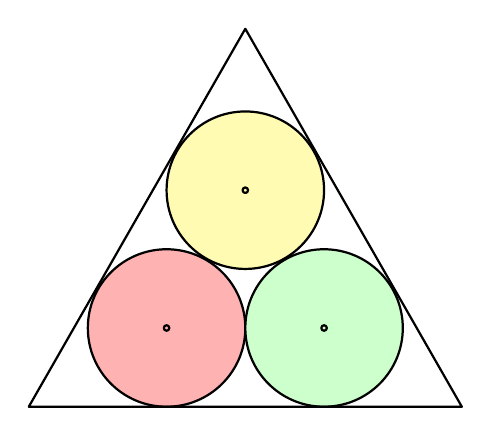
\begin{tikzpicture}[line join=round, line cap=round,thick]
		\draw[fill=red!30] (0,1) arc (0:360:1);
		\draw[fill=green!20] (2,1) arc (0:360:1);
		\draw[fill=yellow!30] (1,2.75) arc (0:360:1);
		\draw (1,1) node[below]{$ $} circle(1pt);
		\draw (-1,1) node[below]{$ $} circle(1pt);
		\draw (0,2.75) node[below]{$ $} circle(1pt);
		\draw (0,4.8) -- (-2.75,0) -- (2.75,0) -- (0,4.8);
		\end{tikzpicture}}
	\loigiai{
		\begin{center}
			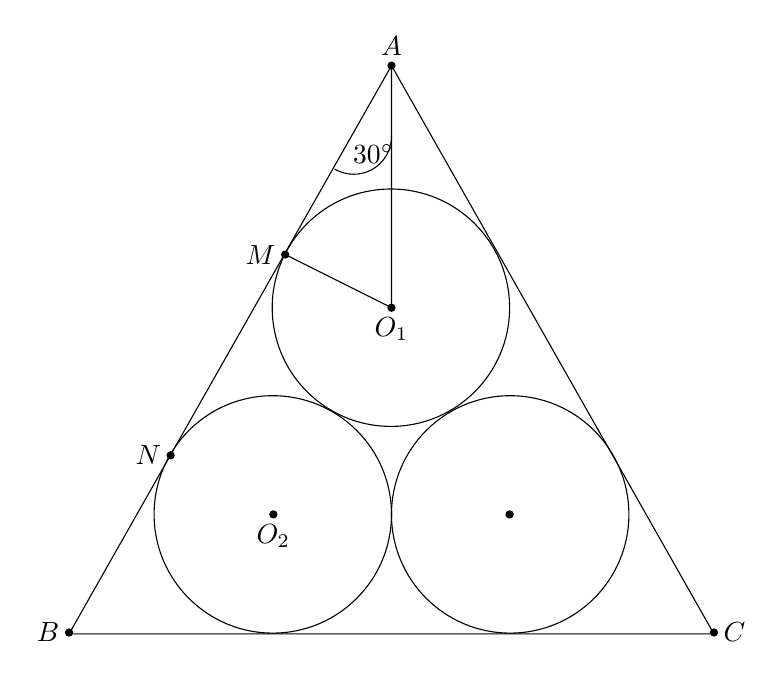
\begin{tikzpicture}[line join=round, line cap=round, scale=1.5]
			\draw (0,1) arc (0:360:1.005);
			\draw (2.01,1) arc (0:360:1.005);
			\draw (1,2.75) arc (0:360:1.005);
			\draw (0,4.2) arc (0:-120:0.32);
			\fill (0,4.8) node[above]{$A$} circle(1pt);
			\fill (-2.73,0) node[left]{$B$} circle(1pt);
			\fill (2.73,0) node[right]{$C$} circle(1pt);
			\fill (1,1) node[below]{$ $} circle(1pt);
			\fill (-1,1) node[below]{$O_2$} circle(1pt);
			\fill (-0.9,3.2) node[left]{$M$} circle(1pt);
		\fill (-1.87,1.5) node[left]{$N$} circle(1pt);
			\fill (0,2.75) node[below]{$O_1$} circle(1pt);
			\draw (0.1,4.05) node[left]{$30^{\circ}$};
			\draw (0,4.8) -- (-2.73,-.012) -- (2.73,-0.012) -- (0,4.8);
			\draw (0,4.8) -- (0,2.75) -- (-0.9,3.2);
			\end{tikzpicture}
		\end{center}
		Ta có, cạnh đáy của hình lăng trụ bằng
		$AB=AM+MN+NB=2AM+O_1O_2=2AM+2$.\\
		Mặt khác, trong tam giác vuông $AMO_1$ có $AM=\dfrac{O_1M}{\tan {{30}^{\circ }}}=\sqrt{3}$.\\
		Suy ra $AB=2( \sqrt{3}+1 )\Rightarrow {S_{\Delta ABC}}=\dfrac{AB^2\sqrt{3}}{4}=\sqrt{3}{{( \sqrt{3}+1 )}^2}$.\\
		Thể tích khối lăng trụ đều là $V_1=S_{\triangle ABC}\cdot h=10\sqrt{3}{{( \sqrt{3}+1 )}^2}$.\\
		Thể tích một thiết bị có dạng khối trụ là $V_2=\pi \cdot {{1}^2}\cdot 10=10\pi $.\\
		Vậy thể tích của phần không gian trống trong thùng hàng là\\
		$V=V_1-3V_2=10\sqrt{3}{{( \sqrt{3}+1 )}^2}-30\pi \approx 35{,}03$ m$ ^3 $.
	}
\end{ex}
%câu 27
\begin{ex}%[DuAn16-SoHaiPhong-NguyenTruongVinh]%[2D1Y2-2]
	Cho hàm số $y=f( x )$ có bảng biến thiên như hình vẽ.
	\begin{center}
				
\begin{tikzpicture}
		\tkzTab		[lgt=1.2,espcl=2.5,nocadre] 
		{$x$/0.6, $f’(x)$/0.6, $f(x)$/2}
		{$-\infty$, $-1$, $3$, $+\infty$}
		{,+,0,-,0,+,}
		{-/ $-\infty$, +/ $5$, -/ $1$, +/ $+\infty$} 
		\end{tikzpicture}
	\end{center}
	Giá trị cực tiểu của hàm số bằng 
	\choice
	{\True $1$}
	{$3$}
	{$5$}
	{$-1$}
	\loigiai{
		Từ có bảng biến thiên của hàm số $y=f( x )$ ta thấy giá trị cực tiểu của hàm số bằng $1$.
	}
\end{ex}
%câu 28
\begin{ex}%[DuAn16-SoHaiPhong-NguyenTruongVinh]%[2D1K5-2]
	\immini{Cho hàm số $y=f( x )$ có đồ thị của hàm số $f’( x )$ như hình vẽ. Biết $f( 0 )=0$. Hỏi hàm số $g( x )=\left| \dfrac{1}{3}f( x^3 )-2x \right|$ có bao nhiêu điểm cực trị?
	\choice
	{\True $3$}
	{$4$}
	{$5$}
	{$1$}
}{
	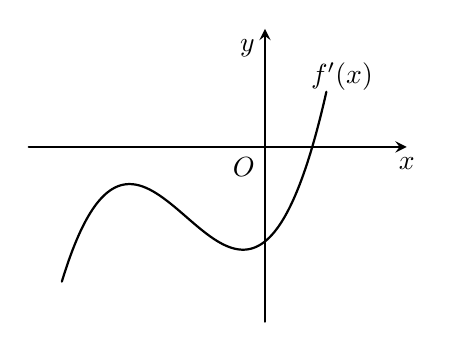
\begin{tikzpicture}[line join=round, line cap=round,>=stealth,thick,scale=0.6]
		\tikzset{label style/.style={font=\footnotesize}}
		\draw[->] (-5,0)--(3,0) node[below] {$x$};
		\draw[->] (0,-3.7)--(0,2.5) node[below left] {$y$};
		\draw (0,0) node [below left] {$O$};
		\draw (2.5,2) node [below left] {$f'(x)$};
		\begin{scope}
			\clip (-5,-3) rectangle (3.6,1.5);
			\draw[samples=200,domain=-4.3:1.3,smooth,variable=\x] plot (\x,{ 0.2*(\x )*(\x+4 )*(\x+1 )-2 });
		\end{scope}
	\end{tikzpicture}
}
	\loigiai{
		Xét hàm số $h( x )=\dfrac{1}{3}f( x^3 )-2x$.\\
		Ta có $h( 0 )=0;$ ${h}’( x )=x^2f’( x^3 )-2;$ ${h}’( 0 )=-2;$
		${h}’( x )=0\Leftrightarrow x^2f’( x^3 )-2=0 \Leftrightarrow f’( x^3 )=\dfrac{2}{x^2}$ $( 1 )$.\\
		Với $x\in ( -\infty ;0 )\Rightarrow  x^3\in ( -\infty ;0 )\,\Rightarrow f’( x^3 )<0$, mà $\dfrac{2}{x^2}>0$ suy ra $( 1 )$ vô nghiệm trên $( -\infty ;0 )$.\\ 
		Với $x\in ( 0;+\infty )\Rightarrow x^3\in ( 0;+\infty )$: $f’( x^3 )$ đồng biến mà hàm số $y=\dfrac{2}{x^2}$ nghịch biến nên phương trình $( 1 )$ có không quá $1$ nghiệm.\\
		Từ đồ thị ta có $( 1 )$ có đúng $1$ nghiệm $x=x_0>0$ hay ${h}’( x )=0$ có đúng $1$ nghiệm $x=x_0>0$.\\ 
		\begin{center}
			
\begin{tikzpicture}[>=stealth]
			\tkzTabInit[lgt=1.2,espcl=3.5,nocadre]
			{$x$ /.7, $h’(x)$ /0.7,$h(x)$ /2.5}
			{$-\infty$,$x_0$,$+\infty$}
			\tkzTabLine{,-, 0,+, }
			\tkzTabVar{+/$-\infty$,-/$h(x_0) $,+/$+\infty $}
			\tkzTabVal{1}{2}{0.5}{$0$}{$0$}
			\end{tikzpicture}
		\end{center}
		Từ đó ta có $h( x_0 )<0$ nên phương trình $h( x )=0$ có hai nghiệm thực phân biệt.\\
		Mặt khác $g( x )=\left| h( x ) \right|=\heva{
			& h( x ),\,\,\quad \text{khi}  \quad h( x ) \ge 0 \\ 
			& -h( x ), \, \text{khi} \quad h( x )<0.}$ \\ 
		Suy ra hàm số $g( x )$ có $3$ điểm cực trị.
	}
\end{ex}
%câu 29
\begin{ex}%[DuAn16-SoHaiPhong-NguyenTruongVinh]%[2D4Y1-1]
	Cho số phức $z$ thỏa mãn $2z+3i=iz+1$, khi đó mô-đun của $z$ bằng 
	\choice
	{$2$}
	{\True $\sqrt{2}$}
	{$\sqrt{5}$}
	{$5$}
	\loigiai{
		Ta có $2z+3i=iz+1\Leftrightarrow ( 2-i )z=1-3i\Leftrightarrow z=\dfrac{1-3i}{2-i}=1-i\Rightarrow \left| z \right|=\sqrt{2}$.
	}
\end{ex}
%câu 30 
\begin{ex}%[DuAn16-SoHaiPhong-NguyenTruongVinh]%[2H3B3-2]
	Trong không gian $Oxyz,$ cho điểm $M( 1;0;0 )$ và hai mặt phẳng $( P )\colon x+y+z+1=0$, $( Q )\colon 2x+y-z=0$. Đường thẳng $(d)$ đi qua điểm $M$ và song song với hai mặt phẳng $( P ),( Q )$ có phương trình là
	\choice
	{$\dfrac{x-1}{-2}=\dfrac{y}{3}=\dfrac{z}{1}$}
	{$\dfrac{x+1}{2}=\dfrac{y+3}{3}=\dfrac{z+1}{1}$}
	{$\dfrac{x-1}{-2}=\dfrac{y}{-3}=\dfrac{z}{1}$ }
	{\True $\dfrac{x-1}{2}=\dfrac{y}{-3}=\dfrac{z}{1}$}
	\loigiai{
		Mặt phẳng $( P )$ có véc-tơ pháp tuyến là $\overrightarrow{n_{P}}=( 1;1;1 )$.\\
		Mặt phẳng $( Q )$ có véc-tơ pháp tuyến là $\overrightarrow{n_{Q}}=( 2;1;-1 )$.\\
		Đường thẳng $(d)$ song song với hai mặt phẳng $( P ),( Q )$ có véctơ chỉ phương là $[\overrightarrow{n_{P}},\overrightarrow{n_\text{Q}} ]=( -2;3;-1 )$.
		Vậy đường thẳng $(d)$ đi qua  điểm $M( 1;0;0 )$ và nhận $\overrightarrow{a} =( -2;3;-1 )$ làm véc-tơ chỉ phương có phương trình là $(d)\colon \dfrac{x-1}{2}=\dfrac{y}{-3}=\dfrac{z}{1}$.
	}
\end{ex}


\begin{ex}%[2D2B6-1]%Câu 31.
Tập nghiệm của bất phương trình $ \log_2 x<2 $ là
\choice
{$ \left( 4;+\infty \right) $}
{$ \left( 0;1 \right) $}
{\True $ \left( 0;4 \right) $}
{$ \left( -\infty;4 \right) $}
\loigiai{
Ta có $ \log_2 x<2 \Leftrightarrow \heva{&x>0\\&x<2^2}\Leftrightarrow 0<x<4 $.\\
Vậy tập nghiệm của bất phương trình là $ S=\left( 0;4 \right) $.
}
\end{ex}
\begin{ex} %[2D2Y1-2] % Câu 32.
	Viết biểu thức $ \sqrt[3]{x\sqrt[4]{x}}=x^{\tfrac{m}{n}} $	với  $ m $,  $ n $ là các số nguyên dương nguyên tố cùng nhau. Khi đó $ m+n $  bằng
\choice 
{$ 13 $}
{\True $ 17 $}	
{ $ 9 $}	
{ $ 8 $}
\loigiai{
Ta có $ \sqrt[3]{x\sqrt[4]{x}}=\sqrt[3]{x\cdot x^{\tfrac{1}{4}}}=\sqrt[3]{x^{\tfrac{5}{4}}}=x^{\tfrac{5}{12}}$.
 Nên $ m=5 $ và $ n=12 $.\\
Vậy $ m+n=17 $.
} 
\end{ex}
\begin{ex} %[2D2Y2-1] %Câu 33.	
Tập xác định của hàm số hàm số $ y=x^{-3} $  là
\choice
{$ \left( 0;+\infty \right) $}
{$ \mathbb{R} $}
{$ \mathbb{R}\setminus \left\lbrace \pm 1 \right\rbrace  $}
{\True $ \mathbb{R}\setminus \left\lbrace 0 \right\rbrace  $}
\loigiai{
Hàm số xác định khi và chỉ khi $ x\neq 0 $.\\
Vậy tập xác định $ \mathscr{D}=\mathbb{R}\setminus \left\lbrace 0 \right\rbrace   $.
}
\end{ex}
\begin{ex}%[2D1Y5-4] %Câu 34.
	Giao điểm của đồ thị hàm số $ y=\dfrac{x-2}{2x-1} $ với trục tung có tọa độ là
\choice 
{ $\left(\dfrac{1}{2}; 0\right)$}
{\True  $\left( 0; 2 \right)$}
{ $\left( 0;-2 \right)$}
{ $\left( 2; 0 \right)$}
\loigiai{
Đồ thị hàm số $ y=\dfrac{x-2}{2x-1} $  giao với trục tung tại điểm có hoành độ $ x=0 $  suy ra $ y=2 $.\\
Vậy giao điểm có tọa độ  $\left( 0; 2 \right)$.
}
\end{ex}
\begin{ex} %[2D4B1-1]%Câu 35.	
Phần ảo của số phức $ z=2-3i $ bằng
\choice
{\True $ -3 $}
{$ 2 $}
{$ 3i $}
{$ 3 $}
\loigiai{
Theo định nghĩa số phức $ z=2-3i $  có phần thực  $ 2 $ là và phần ảo  $ -3 $.
}
\end{ex}
\begin{ex}%[2D1B2-1] %Câu 36.
	Hàm số nào dưới đây có cực trị?
\choice
{$ y=-2x+1 $}
{\True $ y=x^3-3x $}
{$ y=\dfrac{2x+1}{x+1} $}
{$ y=x^3+x $}	
\loigiai{
\begin{itemize}
	\item Hàm số $ y=-2x+2\Rightarrow y'=-2<0,\; \forall x\in \mathbb{R} $. Loại.
	\item Hàm số $y=x^3-3x $ liên tục và xác định trên $ \mathbb{R} $, có $  y'= 3x^2-3 $; $ y'=0\Leftrightarrow\hoac{&x=1\\&x=-1.} $\\
	Bảng xét dấu của $ y' $: \\
	\centerline{% Cần khai báo \usepackage{tkz-tab}
		
\begin{tikzpicture}
			\tkzTabInit[nocadre=true,lgt=2,espcl=2,deltacl=0.5]{$x$/1 ,$y'$/1}
			{$-\infty$ , $-1$ , $1$ , $+\infty$}
			\tkzTabLine{  , + , z ,  - , z , +, }
		\end{tikzpicture}
	}
Dựa vào bảng xét dấu $ \Rightarrow $ hàm số có $ 2 $ điểm cực trị.
\item Hàm số $ y=\dfrac{2x+1}{x+1}\Rightarrow y'=\dfrac{1}{\left( x+1 \right)^2}>0,\;\forall x\neq 1 $. Loại.
\item Hàm số $ y=x^3+x \Rightarrow y'=3x^2+1>0,\;\forall x\in \mathbb{R}$. Loại.
\end{itemize}
}
\end{ex}
\begin{ex}%[2H3K3-6]   %Câu 37.
	Cho mặt phẳng $ ( P )\colon x+2y+2z+1=0 $  và $ A(0;0;1) $; $ B(2;3;7) $. Hình chiếu vuông góc của đoạn thẳng $ AB $  trên mặt phẳng  $ (P) $ có độ dài bao nhiêu?
\choice
{\True $ \dfrac{\sqrt{41}}{3} $}
{$ 2\sqrt{10} $}
{$ \dfrac{\sqrt{41}}{7} $}
{$ \dfrac{20}{3} $}
\loigiai{
$ \bullet $ Cách $ 1 $:\\
Gọi $ I $, $ H $ lần lượt là hình chiếu vuông góc của điểm $ A,\,B $ lên mặt phẳng  $ (P) $.\\
$ \Delta  $ là đường thẳng đi qua $ A $ và vuông góc với $ (P) \Rightarrow \Delta\colon \heva{&x=t\\&y=2t\\&z=1+2t}$; $ t\in \mathbb{R} $.\\
$ I\in \Delta\Rightarrow I\left( t;2t;1+2t \right) $ mà $ I\in (P)\Rightarrow t+2\cdot 2t+2\cdot \left( 1+2t \right)+1=0\Leftrightarrow t=-\dfrac{1}{3}\Rightarrow I\left( -\dfrac{1}{3};-\dfrac{2}{3};\dfrac{1}{3} \right) $.\\
$ \Delta'  $ là đường thẳng đi qua $ B $ và vuông góc với $ (P) \Rightarrow \Delta'\colon \heva{&x=2+m\\&y=3+2m\\&z=7+2m}$; $ m\in \mathbb{R} $.\\
$ H\in \Delta\Rightarrow H\left( 2+m;3+2m;7+2m \right) $.\\
Mà $ H\in (P)\Rightarrow \left( 2+m \right)+2\cdot \left( 3+2m \right)+2\cdot \left( 7+2m \right)+1=0\Leftrightarrow m=-\dfrac{23}{9}\Rightarrow H\left( -\dfrac{5}{9};\dfrac{19}{9};\dfrac{17}{9} \right) $.\\
Vậy hình chiếu vuông góc của đoạn $ AB $ trên mặt phẳng $ (P) $ có độ dài $ IH=\dfrac{\sqrt{41}}{3} $.\\
$ \bullet $ Cách $ 2 $:
\immini{Ta có hai điểm $ A,B $  nằm cùng phía đối với mặt phẳng  $ (P) $. Gọi $ H,K $  lần lượt là hình chiếu của $ A,B $  lên  $ (P) $. Khi đó: \\
 $ d\left( A,(P) \right)=1 $; $ d\left( B;(P) \right)=\dfrac{23}{3} $ và $ AB^2=2^2+3^2+6^2=49 $.\\
Gọi $ I $  là hình chiếu của $ A $  lên $ BK $.\\
Khi đó 
 $$HK=AI=\sqrt{AB^2-\left( BK-AH \right)^2}
=\sqrt{49-\left( \dfrac{23}{3}-1 \right)^2}=\dfrac{\sqrt{41}}{3}.$$
}{
\begin{tikzpicture}[>=stealth,line join=round,line cap=round,font=\footnotesize,scale=.8]
\coordinate (H) at (0,0);
\coordinate (K) at (3,0);
\coordinate (A) at ($ (0,0)+(90:2) $);
\coordinate (B) at ($ (K)+(90:5) $);
\coordinate (I) at ($ (A)+(K)-(H) $);
\draw (-3,-1)--(3.5,-1)--(5.5,1)--(3,1) (0,1)--(-1,1)--(-3,-1);
\draw[dashed] (3,1)--(0,1);
\draw (H)--(K)--(B)--(A)--(H) (A)--(I);
\foreach \i \g in {H/-90,K/-90,I/0,A/180,B/90}\path (\i)+(\g:.3)node{$ \i $};
\end{tikzpicture}
}
}
\end{ex}
\begin{ex} %[2D1K2-2]%Câu 38.
Cho hàm số $ y=f(x) $  có đạo hàm liên tục trên $ \mathbb{R} $  và hàm số $ y=f'(x) $  có đồ thị như hình vẽ. Mệnh đề nào sau đây \textbf{đúng}?\\
\centerline{
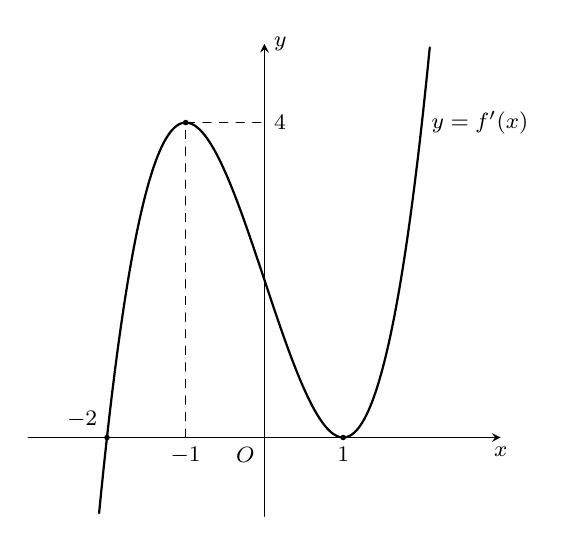
\begin{tikzpicture}[>=stealth,line join=round,line cap=round,font=\footnotesize,scale=1,declare function={f(\x)=(\x-1)^2*(\x+2);}]
\draw[->] (0,-1)--(0,5)node[right]{$y$};
\draw[->] (-3,0)--(3,0)node[below]{$x$};
\draw[thick,samples=150,smooth,domain=-2.1:2.1] plot(\x,{f(\x)});
\draw[dashed] (-1,0)node[below]{$ -1 $}|-(0,4)node[right]{$ 4 $};
\fill 
(-2,0) circle(1pt)
(-1,4)circle(1pt)
(1,0)circle(1pt)
;
\path
(0,0)node[below left]{$ O $}
(2,{f(2)})node[right]{$ y=f'(x) $}
(1,0)node[below]{$ 1 $}
(-2,0)node[above left]{$ -2 $}
;
\end{tikzpicture}}
\choice 
{ Hàm số $y=f(x)$ đạt cực tiểu tại điểm $x=1$}
{ Hàm số $y=f(x)$ đạt cực đại tại điểm $x=-2$}
{ Hàm số $y=f(x)$ đạt cực đại tại điểm $x=-1$}
{\True  Hàm số $y=f(x)$ đạt cực tiểu tại điểm $x=-2$}
\loigiai{
Dựa vào đồ thị ta có bảng biến thiên như sau:\\
\centerline{% Cần khai báo \usepackage{tkz-tab}
	\begin{tikzpicture}[>=stealth]
		\tkzTabInit[nocadre,lgt=1.2,espcl=2,deltacl=0.5]{$x$/.7 ,$f'(x)$/.7,$f(x)$/2}
		{$-\infty$ , $-2$ , $1$ , $+\infty$}
		\tkzTabLine{ , - , $0$ , + , $0$ , + , }
		\tkzTabVar{+/ , -/ }
	\draw  (N23) node[above] (A){}
	(N42) node[below](C){}
	;
	\draw[-stealth] (A.45)--(C);
	\end{tikzpicture}
}
Do đó, hàm số $ y=f(x) $  đạt cực tiểu tại điểm  $ x=-2 $.
}

\end{ex}

\begin{ex} %[2H1K3-2]%Câu 39.
 Cho hình chóp $S. A B C$ có $A B=a, A C=a \sqrt{3}, S B=2 a$ và $\widehat{A B C}=\widehat{B A S}=\widehat{B C S}=90^\circ$. Thể tích của khối chóp $S. A B C$ bằng
\choice 
{ $\dfrac{2 a^3 \sqrt{3}}{9}$}
{ $\dfrac{a^3 \sqrt{6}}{6}$}
{ $\dfrac{a^3 \sqrt{6}}{3}$}
{\True  $\dfrac{a^3 \sqrt{2}}{6}$}
\loigiai{
\immini{
Gọi $ D $ là hình chiếu vuông góc của $ S $ xuống mặt phẳng $ (ABC) $.\\
$ \heva{&SD\perp AB\\
&AD\perp AB}\Rightarrow AB\perp (SAD)\Rightarrow AB\perp AD $.\tagEX{1}
\noindent\\[1mm]
$ \heva{&SD\perp BC\\
	&SC\perp BC}\Rightarrow BC\perp (SCD)\Rightarrow BC\perp CD $.\tagEX{2}\noindent\\[1mm]
Mặt khác $ \widehat{ABC}=90^{\circ} $.\tagEX{3}\noindent
Từ $ (1),(2) $ và $ (3) $ suy ra $ ABCD $ là hình chữ nhật.\\
Trong tam giác vuông $ ABC $, có $ BC=\sqrt{AC^2-AB^2}=a\sqrt{2} $.\\
Trong tam giác vuông $ SBD $, có
}
{\begin{tikzpicture}[>=stealth,line join=round,line cap=round,font=\footnotesize,scale=1]
\coordinate (A) at (0,0);
\coordinate (B) at (3.5,0);
\coordinate (D) at (1.5,1.5);
\coordinate (C) at ($ (B)+(D)-(A) $);
\coordinate (S) at ($ (D)+(90:3) $);
\draw (S)--(A)--(B)--(C)--(S)--(B);
\draw[dashed] (A)--(D)--(C)--cycle (S)--(D)--(B);
\foreach \i \g in {A/-90,B/-90,C/0,D/180,S/90}\path (\i)+(\g:.3)node{$ \i $};
\newcommand{\gocv}[4][black]{\draw[#1] ($(#3)!5pt!(#2)$)--($(#3)!2!($($(#3)!5pt!(#2)$)!.5!($(#3)!5pt!(#4)$)$)$)--($(#3)!5pt!(#4)$);} % Trong cùng hình vẽ chỉ cần sử dụng định nghĩa này một lần
\gocv{B}{A}{S} 
\gocv{A}{B}{C} 
\gocv{S}{C}{B}
\end{tikzpicture}
}
\vspace*{-.3cm}\noindent
 $ SD=\sqrt{SB^2-BD^2}= \sqrt{SB^2-AC^2}=a$.\\
 Khi đó $ B=S_{ABC}=\dfrac{1}{2}AB\cdot BC= \dfrac{a^2\sqrt{2}}{2}$ và $ h=SD=a \Rightarrow V_{S.ABC}=\dfrac{1}{3}Bh=\dfrac{a^3\sqrt{2}}{6}$.
}
\end{ex}
\begin{ex} %[2D2K5-6]%Câu 40.
 Trong gần $ 40 $ năm qua, quỹ đầu tư Berkshire Hathaway của tỷ phú Warren Bufett đạt lợi nhuận trung bình $22,6 \% /$ năm. Tính đến ngày $ 18 $ tháng $ 9 $ năm $ 2020 $, Berkshire Hathaway có vốn hóa thị trường là $ 521,57 $ tỷ đô la, trở thành một trong những công ty đại chúng lớn nhất trên toàn thế giói. Hỏi số vốn ban đầu từ năm $ 1980 $ của quỹ đầu tư Berkshire Hathaway là bao nhiêu với giả thiết khoản lãi hàng năm sẽ được cộng dồn vào tiền vốn ban đầu trong suốt thời gian hoạt động của quỹ?
\choice 
{ \True $ 150,55 $ triệu đô la}
{ $ 12,43 $ tỉ đô la}
{  $ 250,57 $ triệu đô la}
{ $ 57,7 $ tỉ đô la}
\loigiai{
Gọi $ A $ là số vốn ban đầu năm $ 1980 $.\\
Ta có $ 521,57=A\left( 1+22,6\% \right)^{40}\Rightarrow A\approx0,15055 $ (tỷ) $= 150,55 $ (triệu).
}
\end{ex}
\begin{ex}%[2H1B3-2] %Câu 41.
 Cho khối hộp có diện tích đáy $B=7$ và chiều cao $h=6$. Thể tích của khối hộp đã cho bằng
\choice 
{ $42 \pi$}
{\True  $ 42 $}
{ $ 14 $}
{ $14 \pi$}
\loigiai{
Thể tích khối hộp $V=Bh=7\cdot 6=42  $.
}
\end{ex}
\begin{ex}%[1D5K2-1]%Câu 42.
 Đạo hàm của hàm số $y=(1-x)^3$ là
\choice 
{\True  $-3(1-x)^2$}
{ $-(1-x)^3 \ln 3$}
{ $3(1-x)^2$}
{ $(1-x)^3 \ln 3$}
\loigiai{
Ta có $y'=3(1-x)^2\cdot (1-x)'=-3\left( 1-x \right)^2$.
}
\end{ex}


\begin{ex}%[Dự án 16 - TeamTeXHoa - TT Sở Hải Phòng - Võ Thị Thùy Trang]%[2D2K5-5]%43
	Có bao nhiêu giá trị nguyên của tham số $m$ để phương trình $4^{x^2+m}=3^{\ln x+m^2}$ vô nghiệm
\choice
{\True $2$}
{ $0$}
{ $1$}
{ $3$}
\loigiai{
	Điều kiện $x>0$.\\
	Phương trình tương đương $x^2+m=\log _4 3\cdot \left( \ln x+m^2 \right)\Leftrightarrow x^2-\log _4 3\ln x=m^2\log _4 3-m$.\\
	Xét hàm số $f\left( x \right)=x^2-\log _4 3\ln x\Rightarrow f'\left( x \right)=2x-\dfrac{{{\log }_4}3}{x}$.\\
	Ta có $f'\left( x \right)=0\Leftrightarrow x=\dfrac{\sqrt{\log_2 3}}{2}=x_0$.
	\begin{center}
		\begin{center}
			
\begin{tikzpicture}
				\tkzTabInit[nocadre=true,lgt=1.2,espcl=2.5,deltacl=0.6]
				{$x$ /0.6,$f'(x)$ /0.6,$f(x)$ /2}
				{$0$,$x_0$,$+\infty$}
				\tkzTabLine{,-,$0$,+,}
				\tkzTabVar{+/$+\infty$, -/$f(x_0)$,+/$+\infty$}
			\end{tikzpicture}
		\end{center}
	\end{center}
	Để phương trình ${4^{x^2+m}}={3^{\ln x+m^2}}$ vô nghiệm thì $m^2\log_4 3-m<f\left( {x_0} \right)$ mà $m\in \mathbb{Z}\Rightarrow m\in \left\{ 0;1 \right\}$.}
\end{ex}
\begin{ex}%[Dự án 16 - TeamTeXHoa - TT Sở Hải Phòng - Võ Thị Thùy Trang]%[2D3K1-2]%44
		Bằng phép đổi biến số $t=1-x^2$, nguyên hàm $\displaystyle\int \dfrac{x}{1-x^2} \mathrm{\,d}x$ được biến đổi thành nguyên hàm nào dưới đây?
	\choice
	{ $\displaystyle\int{\dfrac{ \mathrm{\,d}t}{t}}$}
	{ $2\displaystyle\int{\dfrac{- \mathrm{\,d}t}{t}}$}
	{\True $\dfrac{1}{2}\displaystyle\int{\dfrac{- \mathrm{\,d}t}{t}}$}
	{ $\dfrac{1}{2}\displaystyle\int{\dfrac{ \mathrm{\,d}t}{t}}$}
	\loigiai{
	Ta có $\displaystyle\int{\dfrac{x}{1-x^2} \mathrm{\,d}x}=\dfrac{-1}{2}\displaystyle\int{\dfrac{-2x}{1-x^2} \mathrm{\,d}x}=\dfrac{-1}{2}\displaystyle\int{\dfrac{ \mathrm{\,d}\left( 1-x^2 \right)}{1-x^2}}=\dfrac{-1}{2}\displaystyle\int{\dfrac{ \mathrm{\,d}t}{t}}$.}
\end{ex}
\begin{ex}%[Dự án 16 - TeamTeXHoa - TT Sở Hải Phòng - Võ Thị Thùy Trang]%[2H3G3-8]%45
		Trong không gian với hệ trục tọa độ $Oxyz$, cho điểm $A\left( 2\ ;\ 1\ ;\ 3 \right)$ và mặt phẳng $\left( P \right)\colon x+my+\left( 2m+1 \right)z-m-2=0$, với $m$ là tham số. Gọi $H\left( a;b;c \right)$ là hình chiếu vuông góc của điểm $A$ trên $\left( P \right)$. Khi khoảng cách từ điểm $A$ đến $\left( P \right)$ lớn nhất,  tính $a+b$.
	\choice
	{ $2$}
	{ $0$}
	{\True $\dfrac{3}{2}$}
	{ $\dfrac{1}{2}$}
	\loigiai{
		Ta có $\mathrm{d}\left( A,\left( P \right) \right)=\dfrac{\left| 2+m+6m+3-m-2 \right|}{\sqrt{1^2+m^2+\left( 2m+1 \right)^2}}=\sqrt{\dfrac{\left( 6m+3 \right)^2}{5m^2+4m+2}}$.\\
		Xét $f\left( m \right)=\dfrac{{{\left( 6m+3 \right)}^2}}{5m^2+4m+2}\Rightarrow f'\left( m \right)=\dfrac{\left( 6m+3 \right)\left( -6m+12 \right)}{{{\left( 5m^2+4m+2 \right)}^2}}=0\Leftrightarrow \left[ \begin{aligned}
			& m=\dfrac{-1}{2} \\
			& m=2. \\
		\end{aligned} \right.$
	\begin{center}
		\begin{center}
			
\begin{tikzpicture}
				\tkzTabInit[nocadre=true,lgt=1.2,espcl=2.5,deltacl=0.6]
				{$x$ /0.6, $y'$ /0.6, $y$ /2.5}
				{$-\infty$,$-0{,}5$,$2$,$+\infty$}
				\tkzTabLine{,-,$0$,+,$0$,-,}
				\tkzTabVar{+/$\dfrac{36}{5}$,-/$0$,+/$\dfrac{15}{2}$,-/$\dfrac{36}{5}$}
			\end{tikzpicture}
		\end{center}
	\end{center}
		Vậy $\max \mathrm{d}\left( A,\left( P \right) \right)=\dfrac{\sqrt{30}}{2}$ khi và chỉ khi $m=2$.\\
		Vậy $\left( P \right)\colon x+2y+5z-4=0$.\\
		Gọi $d$ là đường thẳng qua $A$ và vuông góc $\left( P \right)$ nên $d\colon \heva{& x=2+t\\& y=1+2t\\& z=3+5t}$.\\
		Khi đó $H=d\cap \left( P \right)$.\\
		Ta có $2+t+2+4t+15+25t-4=0\Leftrightarrow 30t=-15\Leftrightarrow t=\dfrac{-1}{2}$.\\
	Suy ra	$H\left( \dfrac{3}{2};0;\dfrac{1}{2} \right)$. Do đó $a+b=\dfrac{3}{2}$.\\
		Cách 2: Khi đó $M\left( x;y;z \right)$ cố định của $\left( P \right)$ thỏa $m\left( y+2z-1 \right)+x+z-2=0,  \forall m$\\
		$\Leftrightarrow \left\{ \begin{aligned}
			& y+2z-1=0 \\
			& x+z-2=0 \\
		\end{aligned} \right. \Rightarrow \Delta \colon  \left\{ \begin{aligned}
			& x=2-t \\
			& y=1-2t \\
			& z=t .\\
		\end{aligned} \right.$\\
		$\left( P \right)$ luôn qua $\left( \Delta \right)$ cố định.
		\begin{center}
				\begin{tikzpicture}[scale=.7,>=stealth, font=\footnotesize, line join=round, line cap=round]
				\node at (2,4) [above]{$A$};
				\node at (0,1.22) [below]{$K$};
				\node at (2,1.8) [below]{$\Delta$};
				\node at (-3.5,0) [above right]{$\left(P\right)$};
%				\clip (-5,-5) rectangle (5,5);
				\draw (-4,0) --(-2,3);
				\draw (-4,0)--(4,0);
				\draw (-1,1)--(3,2);
				\draw (2,4)--(2,2);
				\draw (2,4)--(0,1.22);
%				\tkzDefPoints{2/4/A,2/2/B,3/2/C}
%				\tkzMarkRightAngles[size=0.17](A,B,C)
			\end{tikzpicture}
		\end{center}
		$AH\le AK\Rightarrow d{{\left( A;\left( P \right) \right)}_{\max }}\Rightarrow H\equiv K$.\\
		$K\left( 2-t;1-2t;t \right)\in \Delta$.\\
		 và $\overrightarrow{AK}\cdot \overrightarrow{u_{\Delta}} =0\Rightarrow t=\dfrac{1}{2}\Rightarrow K\left( \dfrac{3}{2};0;\dfrac{1}{2} \right)$.\\
		Suy ra $H\equiv K$ nên $H\left( \dfrac{3}{2};0;\dfrac{1}{2} \right)$.}
\end{ex}
\begin{ex}%[Dự án 16 - TeamTeXHoa - TT Sở Hải Phòng - Võ Thị Thùy Trang]%[2D4G3-2]%46
		Cho số phức $z$ thay đổi thoả mãn $\left| z \right|=\left| z-4-4i \right|$. Gọi $S$ là tập hợp các số phức $w=\dfrac{8z}{\left| {z^2} \right|}$. Biết rằng $w_1,~w_2$ là hai số thuộc $S$ sao cho $\left| w_1-w_2 \right|=2$, khi đó mô-đun của số phức $w_1+w_2-2-2i$ bằng
	\choice
	{ $4$}
	{\True $2$}
	{ $2\sqrt{2}$}
	{ $1$}
	\loigiai{
	Ta có $w=\dfrac{8z}{\left| z^2 \right|}=\dfrac{8z}{\left| z \right|^2}=\dfrac{8z}{z.\overline{z}}=\dfrac{8}{\overline{z}}\Rightarrow \overline{z}=\dfrac{8}{w}$.\\
		Theo giả thiết ta có $\left| z \right|=\left| z-4-4i \right|\Rightarrow \left| \dfrac{8}{\overline{w}} \right|=\left| \dfrac{8}{\overline{w}}-4-4i \right|$\\
		$\Leftrightarrow 8=\left| 8-\left( 4+4i \right)\overline{w} \right|\Leftrightarrow \dfrac{8}{4\sqrt{2}}=\left| 1-i-\overline{w} \right|$
		$\Leftrightarrow \left| w-1-i \right|=\sqrt{2}$.\\
		Đặt $t=w-1-i\Rightarrow \left| t \right|=\sqrt{2}$.\\
		và $\left|t_1-t_2 \right|=\left|w_1-w_2 \right|=2$.\\
		Suy ra $\left| w_1+w_2-2-2i \right|^2=\left| t_1+t_2 \right|^2=2\left( \left|t_1 \right|^2+\left| t_2 \right|^2 \right)-\left| t_1-t_2 \right|^2$
		$=2\left( 2+2 \right)-4=4$.\\
		$\Rightarrow \left| {w_1}+w_2-2-2i \right|=4$.}
\end{ex}
\begin{ex}%[Dự án 16 - TeamTeXHoa - TT Sở Hải Phòng - Võ Thị Thùy Trang]%[2D2Y5-1]%47
	Nghiệm của phương trình $\ln x=1$ là
	\choice
	{ $x=0$}
	{ $x=1$}
	{\True $x=\mathrm{e}$}
	{ $x=\dfrac{1}{\mathrm{e}}$}
	\loigiai{
		Điều kiện $x>0$.\\
		Ta có $\ln x=1\Leftrightarrow x=\mathrm{e}$ (nhận).}
	
\end{ex}
\begin{ex}%[Dự án 16 - TeamTeXHoa - TT Sở Hải Phòng - Võ Thị Thùy Trang]%[1H3B2-3]%48
Cho hình lập phương $ABCD.A'B'C'D'$. Góc giữa hai đường thẳng $AC$ và $DA'$ bằng
\choice
{ $90^\circ $}
{\True $60^\circ $}
{ $30^\circ $}
{ $45^\circ $}
\loigiai{
	\immini{
		Vì $AC\parallel A'C'$ nên góc giữa $AC$ và $DA'$ là góc giữa $A'C'$ và $DA'$.\\
		Xét tam giác $A'C'D$ có $A'C'=C'D=A'D$ nên tam giác $A'C'D$ là tam giác đều.\\
		Vậy góc giữa $A'C'$ và $DA'$ bằng $60^\circ $ hay góc giữa $AC$ và $DA'$ bằng $60^\circ$.
	}
{\begin{tikzpicture}[scale=0.7, font=\footnotesize, line join=round, line cap=round, >=stealth]
		\def\bc{4} % cạnh BC
		\def\ba{2} % cạnh BA
		\def\h{4} % đường cao
		\def\gocB{35} % góc B của đáy
		\coordinate[label=below left:$B$] (B) at (0,0);
		\coordinate[label=above left:$A$] (A) at (\gocB:\ba);
		\coordinate[label=below:$C$] (C) at (\bc,0);
		\coordinate[label=right:$D$] (D) at ($(C)-(B)+(A)$);
		\coordinate[label=above left:$A'$] (A') at ($(A)+(90:\h)$);
		\coordinate[label=left:$B'$] (B') at ($(B)-(A)+(A')$);
		\coordinate[label=below right:$C'$] (C') at ($(C)-(A)+(A')$);
		\coordinate[label=right:$D'$] (D') at ($(D)-(A)+(A')$);
		\draw (B')--(B)--(C)--(D)--(D')--(A')--(B')--(C')--(D') (C)--(C') (D)--(C')--(A');
		\draw[dashed] (A')--(A)--(D) (A)--(B) (A)--(C) (A')--(D);
		\foreach \diem in {A,B,C,D,A',B',C',D'}	\fill (\diem)circle(1.5pt);
\end{tikzpicture}}
}	
\end{ex}
\begin{ex}%[Dự án 16 - TeamTeXHoa - TT Sở Hải Phòng - Võ Thị Thùy Trang]%[2H3K2-7]%49
Trong không gian với hệ trục tọa độ $Oxyz$, cho mặt phẳng $\left( P \right)\colon 2x+y-2z+3=0$ và mặt cầu $\left( S \right)\colon \left( x-1 \right)^2+\left( y-2 \right)^2+\left( z+1 \right)^2=25$. Bán kính của đường tròn giao tuyến của mặt cầu và mặt phẳng bằng
\choice
{ $\sqrt{22}$}
{ $3$}
{\True $4$}
{ $8$}
\loigiai{
	Mặt cầu $\left( S \right)$ có tâm $I\left( 1;2;-1 \right);\,$ bán kính $R=5$.\\
	$\mathrm{d}\left( I;\left( P \right) \right)=\dfrac{\left| 2+2+2+3 \right|}{\sqrt{2^2+1^2+\left( -2 \right)^2}}=3$.\\
	Gọi $r$ là bán kính của đường tròn giao tuyến của mặt cầu và mặt phẳng.\\
	Ta có $r^2+\mathrm{d}^2\left( I;\left( P \right) \right)=R^2$
	$\Leftrightarrow r^2+3^2=5^2$
	$\Rightarrow r=4$.}	
\end{ex}

\begin{ex}%[Dự án 16 - TeamTeXHoa - TT Sở Hải Phòng - Võ Thị Thùy Trang]%[2D1G5-5]%50
	Cho hàm số $y=f\left( x \right)$ liên tục và có đạo hàm cấp hai trên $\mathbb{R}$. Biết rằng đồ thị của các hàm số $y=f\left( x \right),\,y=f'\left( x \right),\,y={f'}'\left( x \right)$ là các đường cong trong hình vẽ bên. Xác định thứ tự các hình
\begin{center}
	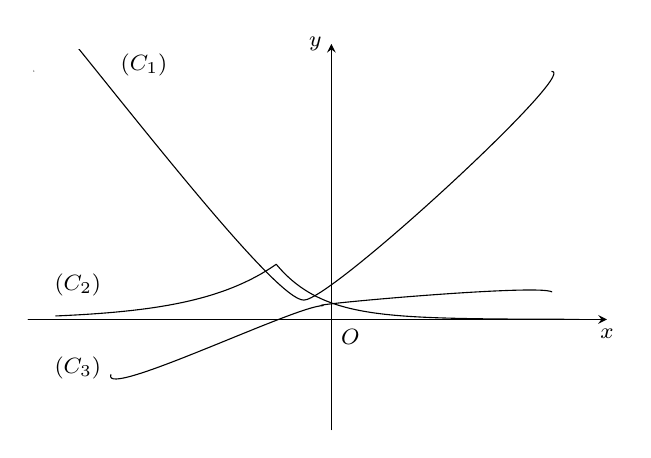
\begin{tikzpicture}[scale=.7,>=stealth, font=\footnotesize, line join=round, line cap=round]
		\def\a{-5/6} \def\b{-5/6} \def\c{9} % Hệ số
		\def\xmin{-5.5} \def\xmax{5}
		\def\ymin{-2} \def\ymax{5}
		%	\draw[color=gray!50,dashed] (\xmin,\ymin) grid (\xmax,\ymax);
		\draw[->] (\xmin,0)--(\xmax,0) node [below]{$x$};
		\draw[->] (0,\ymin)--(0,\ymax) node [left]{$y$};
		\node at (0,0) [below right]{$O$};
		\clip (\xmin+0.1,\ymin+0.1) rectangle (\xmax-0.5,\ymax-0.1);
		\draw 
		(-5.4,4.5)..controls +(120:10) and +(180:1).. (-.5,.35)
		..controls +(0:.5) and +(180:-0.5).. (4,4.5);
		\draw[smooth,samples=300][domain=-5:-1] plot(\x,{2^(\x+1)});
		\draw[smooth,samples=300][domain=-1:5] plot(\x,{0.3^(\x+1)});
			\draw 
		(-4,-1)..controls +(70:-.5) and +(180:.5).. (-0.15,0.25)
		..controls +(0:-0.5) and +(150:0.3).. (4,0.5);
		\node at (-2.8,5) [below left]{$\left(C_1\right)$};
		\node at (-4,1) [below left]{$\left(C_2\right)$};
		\node at (-4,-.5) [below left]{$\left(C_3\right)$};
	\end{tikzpicture}
\end{center}
\choice
{\True $\left( {C_1} \right)\colon y=f\left( x \right),\,\left( {C_3} \right)\colon y=f'\left( x \right),\,\left( {C_2} \right)\colon y={f'}'\left( x \right)$}
{ $\left( {C_3} \right)\colon y=f\left( x \right),\,\left( {C_1} \right)\colon y=f'\left( x \right),\,\left( {C_2} \right)\colon y={f'}'\left( x \right)$}
{ $\left( {C_1} \right)\colon y=f\left( x \right),\,\left( {C_2} \right)\colon y=f'\left( x \right),\,\left( {C_3} \right)\colon y={f'}'\left( x \right)$}
{ $\left( {C_3} \right)\colon y=f\left( x \right),\,\left( {C_2} \right)\colon y=f'\left( x \right),\,\left( {C_1} \right)\colon y={f'}'\left( x \right)$}
\loigiai{
	\begin{itemize}
		\item $\left( {C_1} \right)\colon y=f\left( x \right),\,\left( {C_3} \right)\colon y=f'\left( x \right),\,\left( {C_2} \right)\colon y={f'}'\left( x \right)$ đúng.
		\item 	$\left( C_3 \right)\colon y=f\left( x \right),\,\left( C_1 \right)\colon y=f'\left( x \right),\,\left(C_2 \right)\colon y=f''\left( x \right)$ và 
		$\left(C_3 \right)\colon y=f\left( x \right),\,\left( C_2 \right)\colon y=f'\left( x \right),\break \left( {C_1} \right)\colon y={f'}'\left( x \right)$
		loại vì ${f'}'\left( x \right)>0$ với mọi $x\in \mathbb{R}$ nên$f'\left( x \right)$ phải là hàm số đồng biến trên$\mathbb{R}$, tuy nhiên đồ thị $f'\left( x \right)$ lại có cực trị trên $\mathbb{R}$ nên dẫn đến điều vô lý.
		\item  $\left( {C_1} \right)\colon y=f\left( x \right),\,\left( {C_2} \right)\colon y=f'\left( x \right),\,\left( {C_3} \right)\colon y={f'}'\left( x \right)$
		loại vì nếu ${f'}'\left( x \right)>0$ thì $f'\left( x \right)$ là hàm số nghịch biến nên cũng vô lý.
	\end{itemize}
}
\end{ex}


\Closesolutionfile{ans}
